
\documentclass[twocolumn, a1paper]{article}
 %\usepackage[scale=0.78,size=a1]{beamerposter}
%\setlength{\paperheight}{33.1in}
%\setlength{\paperwidth}{23.4in}
\usepackage{cite}
\usepackage{graphicx}
\usepackage{amsmath}
\usepackage{commath}
\usepackage{adjustbox}
%\usepackage[sc]{mathpazo}
\usepackage[margin=0.5in]{geometry}
%\usepackage{multicol}
\usepackage{mathtools}
\usepackage{abstract}
\usepackage[compact]{titlesec}
\DeclareMathOperator{\sech}{sech}
\newcommand{\matr}[1]{\mathbf{#1}}
%\usepackage{placeins}
%\usepackage{textcomp}
\graphicspath{ {H:/} }

\usepackage{smartdiagram}
\usepackage{metalogo}
\usepackage{dtklogos}



\begin{document}

\title {\textbf{ A Sphere Model for Atrial Fibrillation}}
\author{Tigany Zarrouk \& Mattia Gaggi \textbf{Supervisor}: Kim Christensen \\ Condensed Matter Theory Group---Imperial College London}

\date{}
\maketitle






\section{\textbf{\underline{Introduction}}}

Atrial Fibrillation (AF) is a type of cardiac arrhythmia and one of the major causes of stroke and heart failure. AF is also the most widespread cardiac condition, with over 30 millions of people worldwide suffering from it. In the UK, expenses related to this disease account for more than $1\%$ of the total budget of the National Health Service, which is more than $800$ million pounds.Atrial fibrillation usually manifests itself in patients affected through alterations of the normal cardiac rhythm lasting short periods of time (also called fibrillation episodes).\\

Each heart beat originates as an electric signal in the sinoatrial (SA) node that propagates first into the atria, then through the atrioventricular (AV) node, through Purkinje fibres and finally from the ventricular endocardium to the ventricular epicardium. The electric signal is conducted in the cardiac muscle cells thanks to the polarisation mechanism of the cell membrane. 
When a muscle cell (myocyte) is at rest, there is a built up potential difference between the outside and the inside of the cell (polarisation).





%picture of the heart here



AF is usually produced  by an calcified muscle cells (fibrosis) in the cardiac tissue which generates a process called reentry. During reentry the electric signal wavefront propagation breaks. It has been shown a clear link between fibrosis and AF
Even though many treatments have been developed, the mechanisms behind this condition are not completely understood and AF remains a major topic in medical research. The current research revolves around three possible approaches:


\smartdiagram[bubble diagram]{Current research,
 Physiological \\ models, Image-Based \\ Models, \textbf{ CA Models}, antiarrhythmic \\ drugs) t}
 
 Our research is based on expanding on the wrok done by Kim Christensen on CA (Cellular Automata) models \cite{Christensen}.




\section{\textbf{Kim Christensen Model}}


"Simple Model for Identifying Critical Regions in Atrial Fibrillation"~\cite{Christensen}produced a simple 2D model for AF. The cardiac cells were arranged in a squared grid with horizontal connections, with a percentage of transversal connections (to reproduce the effect of fibrosis) and a percentage of unexcitable cells.

Electric impulse propagation rules:

%insert fucking rules






The results from this model show that there is a threshold value of vertical connections beyond which AF is produced spontaneously (without changing refractory period or conduction speed). This matches real data according to which AF is correlated with fibrosis. 
The model also shows that burning the area affected by AF effectively stops the arrhythmia, which has been recently discovered to be the case . 






\section{\textbf{Implementing Restitution in Kim Christensen Model}} %METHODS

Mechanisms thought to be responsible for active cardiac arrhythmias are either enhanced/abnormal pulse formation or re-entry. For the former, simulations have included modelling the ionic currents of action potentials such as the Fenton-Karma model \cite{Grandi} \cite{Fenton} and modelling the impulse of an action potential using generic reaction-diffusion equations, such as the FitzHugh-Nagumo Model \cite{FitzHugh}. Most of these models are based on the pioneering work of Hodgkin and Huxley who described the action potential of the giant squid axon, which bears similarities to cardiac cells \cite{Hodgkin}. %CHECKKKKKKKKKKKKKKKKKKK
 For all of these models bidomain or monodomain approaches can be used to model the electrical propagation in myocardial tissue. % intracellularly????
  The bidomain model takes into account the anisotropy of intracellular and extracellular spaces. The monodomain model is a reduction of the bidomain model by assuming anisotropy ratios of intracellular and extracellular domains are equal---this is the model most commonly used in simulations today.%ET CETERA?
% ,   is the Many types of models have been used to simulate fibrillatory behaviour in the heart, from, and signals for contraction, to cellular automata and 

Re-entry---the mechanism by which a propagating impulse fails to die out after normal activation of the heart---has been studied in depth via various circus reentry formulations: the Ring Model, the Leading circle model, the Figure-of-Eight model and the Spiral Wave model \cite{Antze} \cite{Tusscher}. The Ring model models a wave of propagation that moves along one, unidirectional pathway of heart tissue and returns to the origin of excitation, thus simulating a central area of inexcitable tissue. This simple model implies that the conduction velocity and the refractory period are both factors: the length of the circuit (pathlength) must be greater or equal to the wavelength (the distance travelled by an impulse during the refractory period). The smaller the wavelength, the greater the number of reentry circuits that can be accommodated during the refractory period to promote fibrillatory behaviour. See figure 2(c).



The Spiral wave model---which consists of a single rotating wavefront around a core, simulating tachycardia---has been observed in systems that have sites that have excited, refractory and resting states in both homogeneous and heterogeneous media \cite{Greenburg} \cite{Bub}. This is due to anisotropies in conduction velocity in the cardiac tissue. See figure 2(b) and figure 3. % for comparison to a normal wavefront. 
 Experimental demonstration of spiral waves has been achieved by in research by Davidenko et al and the concept is now seen to be an underlying driver of fibrillation; the paradigm appears to more closely correspond with many clinical and experimental observations than other models \cite{Davidenko} \cite{Comtois}. In one such observation, the presence of rotors was seen in 96\% of patients with AF, in a 2012 study \cite{afstudy}. The curvature of the spiral wave is related to the speed of the wave, the more curvature the slower the speed of propagation. High curvature, and far-field instability, leads to spiral wave breakage into daughter wavelets. This agrees with
%popular classical modes of thought regarding the initiation of fibrillatory contraction, multiple circuit reentry, which in this case is due to spiral breakup, and 
recent opinions where single, small reentry circuits or local generators have been found to promote fibrillatory activity---the core of the spiral \cite{Skanes} \cite{Nattel2}. The tip of the spiral wave has been seen to drift around the core, thus moving the whole spiral wave. Such meandering can be a factor in promoting fibrillatory activity \cite{Tusscher}.
% Recent observations are in contradiction with the classical viewpoint,  . This is also concurrent 
 Extending the spiral wave model to 3D gives rise to scroll waves which propagate through multiple layers of cells and give rise to more complex wave dynamics and is therefore hard to implement computationally.  %It has been seen that the if a spiral wave is in homogenous media then it will always return to its resting state . 


\begin{figure}
\caption[short title]{Diagram showing a spiral wave reentry circuit. (a), a normal wavefront in the heart. (b) spiral wave, which simulates tachycardia, as can be seen by multiple propagating wavefronts in a small area. (c), turbulent activity due to break up of spiral wave giving rise to fibrillation \cite{Alonso}}
\centering
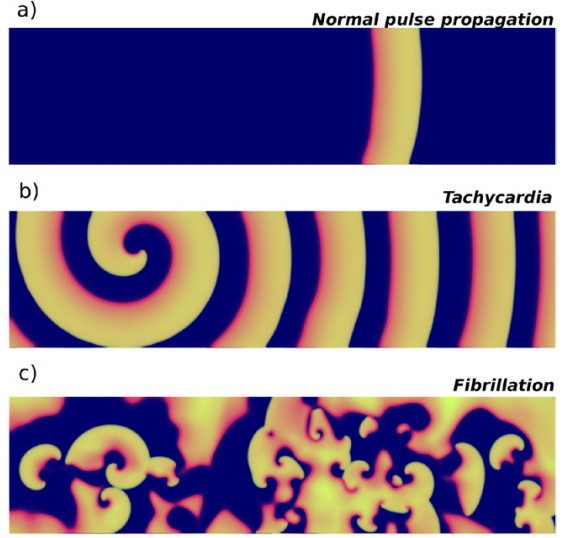
\includegraphics[width = 0.25\textwidth]{spiralbreak2tachy}
\end{figure}

\section{\textbf{Kim Christensen model on a Sphere}}





Recent research has shown that rotating wavefronts can be initiated in regions where the proportion of transverse coupling between strands of tissue is reduced to a critical value, leading to spontaneous fibrillatory activity, in contrast to normal 'linear' wavefronts. This can be seen in the rectilinear cellular automata model developed by Christensen et al and reflects current opinion: the fibrosis of cells, which reduces the coupling of electrical signals to other cells, leads to AF\cite{Christensen}. This research also supports targeted ablation to stop AF. Other studies suggest similar mechanisms such as the coupling of fibroblasts to atrial myocytes heterogeneously gives rise to spiral wave breakups \cite{Ozawa}.


In research by Fedotov, a cellular automaton model was constructed on the surface of a triangulated sphere to model spiral rotor waves on a closed, heterogeneous surface \cite{Fedotov}. It was shown that both a decrease in refractory period and conduction velocity from a "healthy" myocardium state, where no irregular excitation waves above 300bpm are observed, resulted in an area where spiral waves were formed. In addition, a multi-electrode system was created to study the localization of AF sources by simulated electrograms. 


More cellular automata models have been researched by Siregar et al, where a 3D model of the heart, with simplified morphology is simulated and, in addition, a 2D CA model is compared qualitative model \cite{Siregar} \cite{Siregar2}. A hybrid I/O cellular automata approach has also been studied in research by Bartocci et al to describe cardiac tissue and improve the efficiency of the simulation process by parallelization \cite{Bartocci}.

 The impact of left and right atrial tissue electrical heterogeneities to promote AF has been studied in a biophysical model and it was seen that AF is more persistent in the right atria \cite{Luca}. Further development could be achieved by simulation from a cellular automata perspective. Modelling scroll waves and replicating the morphology of the heart with its heterogeneities more closely seem to be viable directions for further research. The effects of antiarrhythmic drugs on the heart during AF can be studied, along with the associated mechanism by which proarrhythmia occurs, and methods for its rectification. Developing ways to find CFAEs with novel electrogram methods via simulation could help targeted ablation, stopping AF more effectively and efficiently. 



% Further developments could be obtained through this parallelization combined with 3D modelling, more accurately depicting the shape of the heart, making the code more efficient.

 %Many of these studies suggest targeted ablation can hinder or fully stop AF, therefore, electrogram-guided ablation to find CFAEs is a promising method it is concurrent with clinical observations. %electrogram-guided ablation to find CFAE.


%Most of these models only work one or two dimensionally, assuming that the heart is a 2D surface and not a 3D




%Cellular automaton models


%MAIN PAPER FROM KIM CHRISTIENSEN
%BIPOLAR ELECTROGRAM??
%METHODS TO POTENTIALLY STOP ATRIAL FIBRILLATION




%FUUUUUUUUUUUUURTHER METHODZZZZZZZZZZZZZZZZZZZZZZZZZZ




%\section{\textbf{\underline{Implications and Discussion}}}  %What our research project will be able to achieve, potentially



%\section{\textbf{\underline{Conclusion}}}




%In this literature review, possible underlying mechanisms of atrial fibrillation (AF) are described along with the relevant the electrophysiology of heart cells, specifically myocytes and  sinoatrial node cells. The integral role of these cells with regards to action potential propagation to contract the heart periodically is described. Models to simulate the action potentials of these cells to simulate reentry are seen to be a computationally costly way of modelling large scale cardiac tissue. Studied models of electrical wavefront propagation (reentry) that could cause AF, such as the ring, leading circle and spiral wave models are described; spiral wave reentry has been observed to be an underlying mechanism. Cellular automata---where cells' states change based on the states of their nearest neighbours---are viable models that reduce the amount of computation by not considering differential equations governing the action potentials. Therefore, reentry can be modelled on a large scale more easily. Moore neighbourhoods used with a Markus model can achieve smooth spiral waveforms that are isotropic and therefore model spiral wave reentry in a cellular automata models effectively. New directions of research can be taken to more accurately model AF such as: the morphology and heterogeneities of the heart, modelling 3D scroll wave dynamics and using hybrid I/O automata. 

\section{\textbf{\underline{Bibliography}}}
\begin{thebibliography}{7}

%####################################################


\bibitem{Comtois}
P. Comtois, J. Kneller, S. Nattel,
\emph{Of circles and spirals: Bridging the gap between the leading circle and spiral wave concepts of cardiac reentry}
Europace. 2005 Sep;7 Suppl 2:10-20.
DOI: http://dx.doi.org/10.1016/j.eupc.2005.05.011



\bibitem{Alonso}
S. Alonso, M. Bar and B. Echebarria
\emph{Nonlinear physics of electrical wave
propagation in the heart: a review},
Rep. Prog. Phys. 79 (2016) 096601, 
doi:10.1088/0034-4885/79/9/096601

\bibitem{Christensen}
Kim Christensen, Kishan A. Manani, and Nicholas S. Peters
\emph{Simple Model for Identifying Critical Regions in Atrial Fibrillation}
Phys. Rev. Lett. 114, 028104 – Published 16 January 2015



\bibitem{Fedotov}
N. M. Fedotov,  A. I. Oferkin, and S. V. Zhary,
\emph{Modeling Sources of Atrial Fibrillation on a Triangulated Sphere}
Biomedical Engineering, Vol. 49, No. 2, July, 2015, pp. 112115. 



%imref https://o.quizlet.com/i/1UZTM_D5PFefI8E5JOk8Ig_m.jpg


\end{thebibliography}


\end{document}